\chapter{Dimensionality reduction}{}

%citazione introduttiva
\epigraph{\textit{We need data, but maybe not all of them.}}{}

Databases, Internet of Things, big data provide tons of data per second. There is an obvious obstacle in processing all of them since a large computational power and a lot of storage memory are needed. Besides, a portion of this data does not provide useful information since it may have a fixed value or an extremely high correlation with the other data. We introduce dimensionality reduction strategies to smooth the process of data processing and to get information fastly and efficiently. These strategies aim at getting the highest level of information possible using the lowest amount of input data.\par

Let assume that data from our sources is organised in a dataset $X_{N\times P}$ having $N$ observation (rows) and $P$ features (columns). Each observation describes the realisation of a phenomenon characterised by the $P$ features. Dimensionality reduction aims at explaining the information of each row in $X$ using only K features, with $K<P$. To meet this goal, features can be:

\begin{itemize}
    \item extracted (i.e. the $P$ features are transformed to explain the majority of the information in $X$);
    \item selected (i.e. a subset $K$ of $P$ explains the majority of the information in $X$). 
\end{itemize}

The following paragraphs explore techniques belonging to these two methodologies.\footnote{The package logproj provides methods to deal with time series \href{https://github.com/aletuf93/logproj/blob/master/logproj/ml_dimensionalityReduction.py}{here}.} 

\section{Feature extraction}
The most common feature extraction strategy is the principal component analysis (PCA); this section introduces it using the singular value decomposition (SVD) to decompose a dataset $X$. SVD and PCA can be used when a learning table is composed of many columns (e.g. with image recognition or dummy columns from an initial dataset containing categorical variables converted into binary features). SVD and PCA use eigenvalues and eigenvector to transform the features space reducing overfitting. Eigenvectors are defined as vectors whose direction does not change when a linear transformation is applied to them. Eigenvalues are the scalar used to transform the eigenvectors. Given a matrix $A$, we can write:

\begin{equation}
Ax-\lambda x=0
\label{eq_eigenvaluesEigenvectors}
\end{equation}
Where x is the eigenvector of A and $\lambda$ are the eigenvalues of A.

\subsection{Singular Value Decomposition (SVD)} \label{secSVD}
In general, any matrix $X_{N,P}$ can be decomposed into a product of a mixing matrix $U_{N,K}$ and a dictionary matrix $V_{P,K}$ such that:
\begin{equation}
X=UV^T
\label{eq_SVD1}
\end{equation}

A row $x_i\in X$ is a linear combination (according to an entry $u_i\in U$) of the linearly independent elements $v_i\in V$. Singular value decomposition (SVD) is a matrix factorisation technique which decomposes a matrix $X$ into:

\begin{equation}
X_{N,P}=U_{N,K}D_{K,K}V_{P,K}^T
\label{eq_SVD2}
\end{equation}

Table \ref{tab_svd} shows the information content of the three matrices produced by the SVD.

% INSERT tab_svd
\begin{figure}[hbt!]
\centering
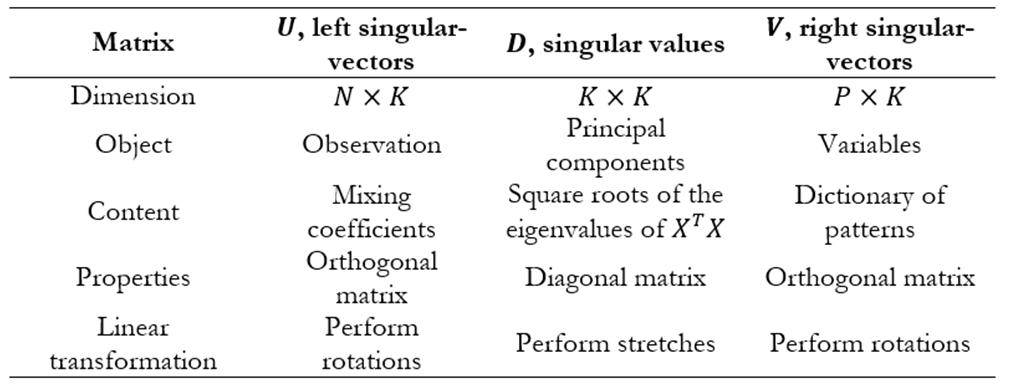
\includegraphics[width=0.9\textwidth]{SectionLetsMath/dimensionalityReduction_figures/tab_svd.png}
\captionsetup{type=table}
\caption{elements of the SVD.}
\label{tab_svd}
\end{figure}

\subsection{Principal Component Analysis (PCA)} \label{secPCA}
PCA aims at reducing  $X_{N,P}$ to $C_{N,K}$  with $K<P$ where $K$ is the number of orthogonal vectors used to explain the variability of $X$. The PCA projects the elements of $X$ in the $K$ directions defined by $V_K$ such that the variance of the $N$ observation is maximised along this direction. In practice, PCA projects the reference system of the $P$ variables onto a new Kdimensional coordinate system $V$. All the entries $x_i$ of the matrix $X_{\left(N,P\right)}$ are converted into the new reference system at $x_{i\left(1,P\right)}^Tv_{\left(P,1\right)}\ $ . PCA defines:

\begin{equation}
v_{\left(P,1\right)}=\arg\max_{v:\left|\left|v\right|\right|=1}{{\frac{1}{N}\sum_{i}\left(x_i^Tv\right)^2}}
\label{eq_PCA}
\end{equation}

It is necessary to remember that, before applying PCA:
\begin{enumerate}
    \item Data has to be centred; i.e. $X=X-{\bar{x}}^T$, since the equation \ref{eq_PCA} maximises the variance of the sample data.
    \item Data has to be standardised;  i.e. having the same variance of all the variables $P$. Otherwise, variables with higher (absolute) variances will overcome the others.
\end{enumerate}

In addition to these, the maximisation objective is constrained to $\left|\left|v\right|\right|=1$ for two reasons:

\begin{enumerate}
    \item We are only interested in the direction of the projection, not in its magnitude;
    \item Without this constraint, the maximisation objective would be unbounded.
\end{enumerate}

Let, now, express the maximisation function at:
\begin{equation}
\arg\max_{v:\left|\left|v\right|\right|=1}{{\frac{1}{N}v^TX^TXv}}
\label{eq_PCA1}
\end{equation}

Please note that the covariance matrix $S_{xx}$ equals $\frac{1}{N}X^TX$, then:

\begin{equation}
\arg\max_{v:\left|\left|v\right|\right|=1}{{v^TS_{xx}v}}
\label{eq_PCA2}
\end{equation}

By using Lagrangian multipliers $\lambda$, it is possible to express the maximisation function at:

\begin{equation}
\max{v^TS_{xx}v-\lambda(v^Tv-1)}
\label{eq_PCA3}
\end{equation}

It is then, possible proceed to calculate the stationary points, i.e. where the derivative of the function (regards to $v$) is equal to zero.

\begin{equation}
\frac{d}{dv}\left\{v^TS_{xx}v-\lambda\left(v^Tv-1\right)\right\}=v^TS_{xx}-\lambda v=0
\label{eq_PCA4}
\end{equation}

\begin{equation}
S_{xx}v=\lambda v
\label{eq_PCA5}
\end{equation}

We conclude that:
\begin{itemize}
    \item $v$ is the eigenvector of $S_{xx}$;
    \item $\lambda$ is the eigenvalue of $S_{xx}$.
\end{itemize}

It is, then, possible to conclude that the variance is maximised when $v$ is an eigenvector of $S_{xx}$ (i.e. the covariance matrix) corresponding to the largest eigenvalue $\lambda$. In practice, the PCA is performed using the sample covariance matrix $S_{xx}=\frac{1}{N-1}X^TX$ and the SDV of $X^TX$.

\begin{equation}
X^TX=\left(UDV\right)^T\left(UDV^T\right)=VD^TU^TUDV^T
\label{eq_PCA6}
\end{equation}
Since $U$ is orthogonal, $U^TU=I$, then:

\begin{equation}
X^TX=VD^TDV^T
\label{eq_PCA7}
\end{equation}

Since $D$ is a square matrix, $D^TD=D^2$, then:
\begin{equation}
\begin{split}
    X^TX=VD^2V^T \\
    V^TX^TXV=D^2 \\
    {\frac{1}{N-1}V}^TX^TXV={\frac{1}{N-1}D}^2 \\
    V^TS_{xx}V={\frac{1}{N-1}D}^2 \\
\end{split}
\label{eq_PCA8}
\end{equation}

Then:
\begin{itemize}
    \item The eigenvectors of $S_{xx}$ are the right-singular vectors $V$;
    \item The eigenvalues $\lambda_k$ (which are the variance of the components) are equal to $\frac{1}{N-1}d_k$, where $d_k$ are the squared singular values.
\end{itemize}

In conclusion, the PCA performs the SVD on the data covariance matrix $S_{xx}$, and it produces three outputs:
\begin{enumerate}
    \item The principal component directions, i.e. the right singular vectors $V_{K,P}$ of an SVD which are the eigenvectors of $X^TX$.
    \item The principal components, i.e. a matrix $C_{N,K}$, obtained projecting $X_{N,P}$ onto the principal components directions $V_{K,P}$ the left singular vectors $U_{N,K}$:
        \begin{equation}
        C_{N,K}=X_{N,P}V_{P,K}=UDV_{N,P}^TV_{P,K}=UD_{N,K}^T
        \label{eq_PCA9}
        \end{equation}
    Accordingly, $U$ (the left-singular value matrix) is the matrix of $u_j$ with the projections of the row vectors of $X$ in the new reference system (direction $v_j$) scaled by $d_j$. In practice, the PCA produces $k$ principal components $(k=1,\ldots,K)$ which are a linear combination of the original variables:
        \begin{equation}
        c_k=x_1u_1+\ x_2u_2+\ldots+x_Pu_P
        \label{eq_PCA10}
        \end{equation}
    \item The variance of each component, given by the eigenvalues $\lambda_k=1,\ldots,K$. This is obtained from the singular values in $D_{K,K}$.
        \begin{equation}
        var\left(c_k\right)=\frac{1}{N-1}d_k^2
        \label{eq_PCA11}
        \end{equation}
\end{enumerate}
	
	
The theory does not explain how to choose the number of PCs. This information can be obtained by building a curve showing the information content of each principal component. Figure \ref{fig_PCAinformation} presents this curve based on the data of the sample \textit{wine dataset}. The curve illustrates the percentage of the variance of the dataset $X$ given a certain number of components $K$. In this case, the dataset $X$ count 13 features, but the first six components are enough to explain 80\% of the variance of $X$.\footnote{The source code of Figure \ref{fig_PCAinformation} is available \href{https://github.com/aletuf93/logproj/blob/master/examples/05.\%20Dimensionality\%20Reduction.ipynb}{here}.
}	

% INSERT fig_PCAinformation
\begin{figure}[hbt!]
\centering
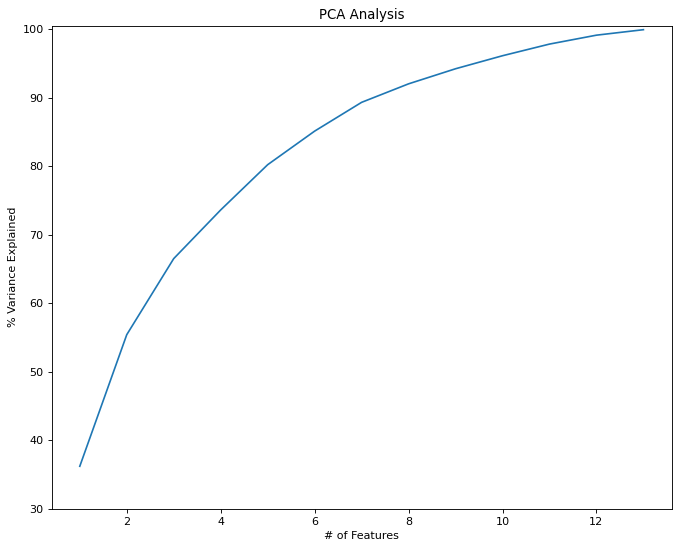
\includegraphics[width=0.8\textwidth]{SectionLetsMath/dimensionalityReduction_figures/fig_PCAinformation.png}
\captionsetup{type=table}
\caption{Cumulative curve of the information content of the principal components.}
\label{fig_PCAinformation}
\end{figure}

\subsection{Multi-dimensional scaling} \label{secMultiDimensionalScaling}
In some cases, we do not have a matrix $X_{N,P}$ with observations and features but a distance matrix $D_{N,N}$ expressing a pairwise distance between each observation, for a given feature. In this case, it is recommendable to turn he $D$ matrix into a $P$ one, but this involves the approximation of the distance values into a $K$-dimensional space.\par

Multidimensional scaling aims at this goal, considering a $D_{N,N}$ and finding a low-dimensional projection of the data such that a stress function is minimised.

\begin{equation}
    \min stress\left(X\right)=\ {\sum_{i\neq j}\left(d_{ij}-\left|\left|x_i-x_j\right|\right|\right)}^2
    \label{eq_MDS}
\end{equation}

\subsection{t-SNE}

t-SNE is a common technique when the number of features $P$ is high. This technique tries to separate the variables rather than combining their effect (as in PCA); also, it provides effective visualisation in low dimensional space (e.g., $K=2$).\par

t-SNE algorithm proceeds step by step, determining the similarity between each observation of the dataset $X$ according to the values of its features $P$. The similarity is measured as the distance between each observation and a Gaussian curve which is, then normalised to 1. Once all similarity values are calculated, a similarity matrix $D$ is defined.\par

All the observation are randomly scattered on the $K$-dimensional space, and their distance is measured as the distance between the observation and a $t$-distribution populating the matrix $D_t$. At this stage, points are re-organised in the $K$-dimensional space one by one to make $D_t$ similar to $D$ defining compact clusters.

\section{Feature selection}
Feature selection strategies implement heuristics to define a subset of the P features to train learning algorithms. The following paragraphs illustrate these strategies.

\subsection{Selection by correlation}
The correlations between the features of the input dataset $X$ are values to check carefully before training a learning algorithm. If two features are highly correlated, it may be necessary to exclude one of them since the other already describes the variability of the dataset. The correlation matrix is used for this purpose to identify the correlation coefficients of all the possible couples of variables. Figure \ref{fig_corrMatrix} shows an example of a correlation matrix from the wine dataset using different colour gradients to highlight positive and negative correlations.\footnote{The source code of Figure \ref{fig_corrMatrix} is available \href{https://github.com/aletuf93/logproj/blob/master/examples/05.\%20Dimensionality\%20Reduction.ipynb}{here}.}

% INSERT fig_corrMatrix
\begin{figure}[hbt!]
\centering
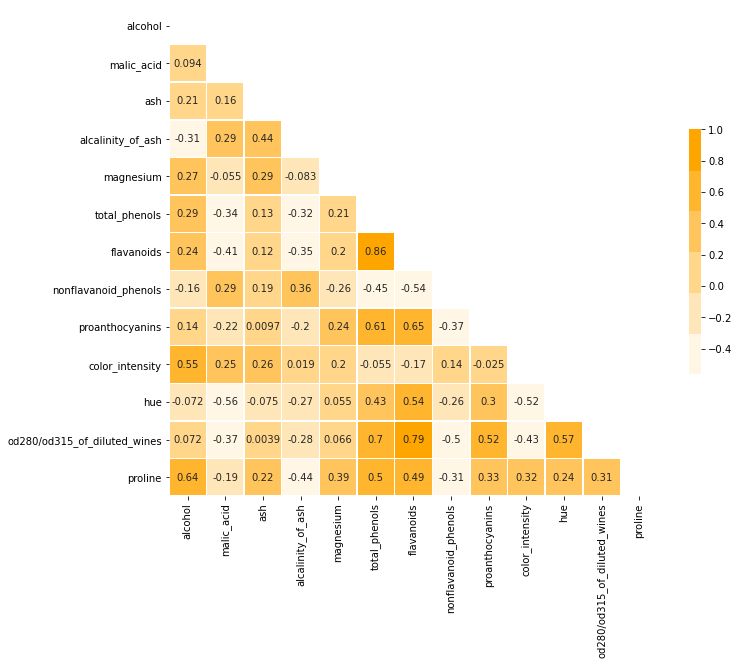
\includegraphics[width=0.8\textwidth]{SectionLetsMath/dimensionalityReduction_figures/fig_corrMatrix.png}
\captionsetup{type=table}
\caption{Correlation matrix of the wine dataset.}
\label{fig_corrMatrix}
\end{figure}

Another strategy based on the correlation consists of training an algorithm only with a subset of variables having a minimum value of correlation with the target variable. Figure \ref{fig_selectCorr} shows the correlation behaviour of the features of the \textit{wine dataset} with the target variable. The plot shows the number of features (y-axis) having a minimum correlation value (x-axis) with the target variable. One may decide to set a threshold of minimum correlation to work with a subset o variable resulting significantly correlated to the target variable (e.g. at least 30\% of correlation).\footnote{The source code of Figure \ref{fig_selectCorr} is available \href{https://github.com/aletuf93/logproj/blob/master/examples/05.\%20Dimensionality\%20Reduction.ipynb}{here}.}

% INSERT fig_selectCorr
\begin{figure}[hbt!]
\centering
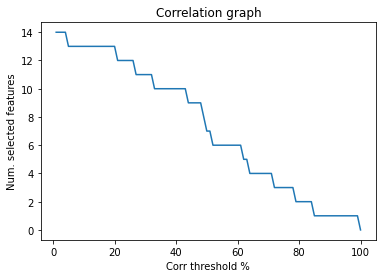
\includegraphics[width=0.8\textwidth]{SectionLetsMath/dimensionalityReduction_figures/fig_selectCorr.png}
\captionsetup{type=table}
\caption{Number of features with a minimum correlation threshold with the target variable (wine dataset).}
\label{fig_selectCorr}
\end{figure}

\subsection{Selection by variance}
Another strategy is to select a subset of variables whose variance is above a certain level. The idea is the following: if a feature has a low variance, it does not add too much information to the dataset. All the features with variance equal to zero should be removed since they do not add any information to the dataset. Figure \ref{fig_selectVariance} illustrates the variance of the features of the \textit{wine dataset}. The majority of the features has a variance lower than 60\%.\footnote{The source code of Figure \ref{fig_selectVariance} is available \href{https://github.com/aletuf93/logproj/blob/master/examples/05.\%20Dimensionality\%20Reduction.ipynb}{here}.}

% INSERT fig_selectVariance
\begin{figure}[hbt!]
\centering
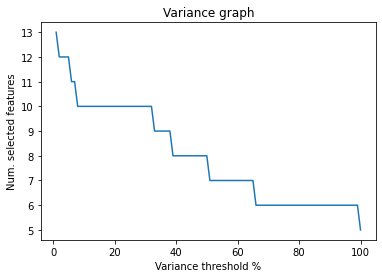
\includegraphics[width=0.8\textwidth]{SectionLetsMath/dimensionalityReduction_figures/fig_selectVariance.png}
\captionsetup{type=table}
\caption{Number of features above a minimum variance threshold (wine dataset).}
\label{fig_selectVariance}
\end{figure}

\subsection{Selection by Lasso coefficients}
Lasso regression (further details in Section \ref{secLassoRegression}) is a prediction model that extends the linear regression which embeds a feature selection strategy. It automatically identifies a coefficient for each feature, shrinking the feature according to its relative importance. The coefficients of a Lasso regression can be used to select only the important features. Figure \ref{fig_LassoPath} shows the graph with the feature coefficients of the \textit{wine dataset} (on the y-axis) depending on the tuning hyperparameter $\alpha$ of the Lasso on the x-axis and the value of the coefficients.\footnote{The source code of Figure \ref{fig_LassoPath} is available \href{https://github.com/aletuf93/logproj/blob/master/examples/05.\%20Dimensionality\%20Reduction.ipynb}{here}.} 

% INSERT fig_LassoPath
\begin{figure}[hbt!]
\centering
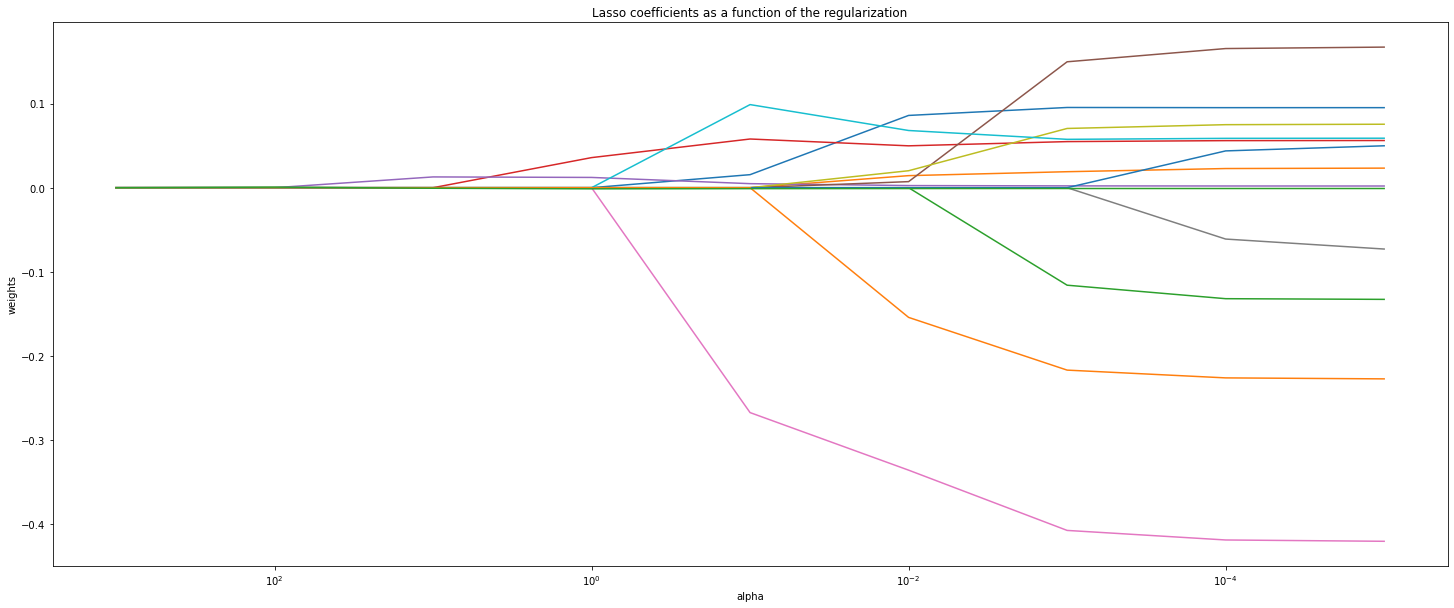
\includegraphics[width=0.8\textwidth]{SectionLetsMath/dimensionalityReduction_figures/fig_LassoPath.png}
\captionsetup{type=table}
\caption{Lasso shrinkage coefficients graph depending on the value of the hyperparameter $\alpha$ (wine dataset).}
\label{fig_LassoPath}
\end{figure}

The graph shows that many coefficients are kept to zero up to some values of $\alpha$. Features can be selected using Lasso identifying a minimum threshold on the value of the coefficients, pinpointing relative importance of the underlying attributes. Figure \ref{fig_selectLasso} illustrated the number of features selected from the \textit{wine dataset} by using different thresholds on the value of the coefficients.\footnote{The source code of Figure \ref{fig_selectLasso} is available \href{https://github.com/aletuf93/logproj/blob/master/examples/05.\%20Dimensionality\%20Reduction.ipynb}{here}.} 


% INSERT fig_selectLasso
\begin{figure}[hbt!]
\centering
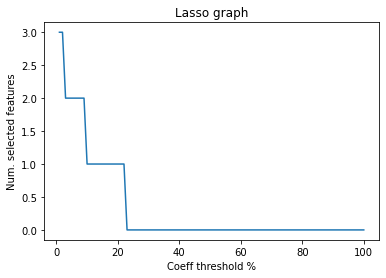
\includegraphics[width=0.8\textwidth]{SectionLetsMath/dimensionalityReduction_figures/fig_selectLasso.png}
\captionsetup{type=table}
\caption{Number of features above a minimum lasso coefficient threshold (wine dataset).}
\label{fig_selectLasso}
\end{figure}

\subsection{Selection by using a decision tree}
A decision tree trains a predicting model branching on the value of a variable defining a tree structure (further details in Section \ref{secDecisionTrees}). The most important features can be selected, evaluating which of them appears the most as a branching variable. Identifying a minimum threshold on the number of times a feature appears as a branching variable works as a feature selection strategy.

\subsection{Forward Stepwise selection}

Forward stepwise selection uses the principles of the linear regression (see section \ref{secLinearRegression}) to identify the most relevant features. There are other algorithms based on the linear regression to select features (e.g. best subset selection, forward stagewise selection) but forward stepwise has been chosen since it can be efficiently implemented compared to the others. The residual sum-of-squares (RSS) of linear regression is always minimised when the number of predictors is maximum. Nevertheless, this does not imply a low bias and variance (affecting the prediction error). For this reason, we want to select a subset of the initial features to reduce the probability of overfitting. Forward stepwise selection works as follows.

\begin{algorithm}[H]
\DontPrintSemicolon
\SetAlgoLined
Identify the intercept of the linear regression\;
\For{i=1:number of features of the dataset}{
    Select one feature improving the most the fit of the model \;
    Add the feature to the model \;
}

\caption{Forward Stepwise algorithm} \label{secForwardStepwise}
\label{algo_forwardStepwise}
\end{algorithm}

Figure \ref{fig_selectForwardStepwise} shows the outcome of the forward stepwise regression of the wine dataset. Increasing the number of features, the RSS decreases and the $r^2$ of the model increases. Besides, a relatively small number of feature (i.e. the first five features) is enough to fit the linear model obtaining a relatively small error. \footnote{The source code of Figure \ref{fig_selectForwardStepwise} is available \href{https://github.com/aletuf93/logproj/blob/master/examples/05.\%20Dimensionality\%20Reduction.ipynb}{here}.} 

% INSERT fig_selectForwardStepwise
\begin{figure}[hbt!]
\centering
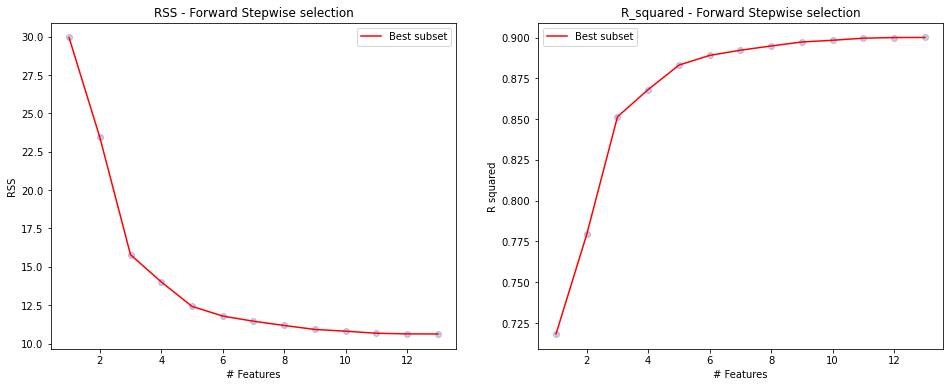
\includegraphics[width=1\textwidth]{SectionLetsMath/dimensionalityReduction_figures/fig_selectForwardStepwise.png}
\captionsetup{type=table}
\caption{Forward stepwise selection graph applied to the wine dataset.}
\label{fig_selectForwardStepwise}
\end{figure}

\section*{Further reading}
Supplementary reading materials can be found in \cite{Dinov2018}.

%\clearpage
\bibliographystyle{ieeetr}
\bibliography{SectionLetsMath/dimensionalityReduction_ref}




